\documentclass[11pt]{article}
\usepackage{amsmath}
%\usepackage{extsizes}
\usepackage{amsmath,amssymb}
%\usepackage{omegavn,ocmrvn}
%\usepackage[utf8x]{inputenc}
\usepackage[utf8]{vietnam}

\usepackage{longtable}
\usepackage{answers}
\usepackage{graphicx}
\usepackage{array}
\usepackage{pifont}
\usepackage{picinpar}
\usepackage{enumerate}
\usepackage[top=3.0cm, bottom=3.5cm, left=3.5cm, right=2.5cm] {geometry}
\usepackage{hyperref}


\newtheorem{bt}{Câu}
\newcommand{\RR}{\mathbb R}
\Newassociation{sol}{Solution}{ans}
\newtheorem{ex}{Câu}
\renewcommand{\solutionstyle}[1]{\textbf{ #1}.}
\newcommand{\m}[1]{
	\begin{bmatrix}
		#1
	\end{bmatrix}
}

\begin{document}
% \noindent
\begin{tabular*}
{\linewidth}{c>{\centering\hspace{0pt}} p{.7\textwidth}}
Trường ĐHKHTN, ĐHQGHN & {\bf Học Kỳ 1 (2018-2019)}
\tabularnewline
K61 TTƯD & {\bf Bài kiểm tra thường xuyên \\ Đề I \& II \\ Đề còn đang dang dở và 0 tốt}
\tabularnewline
\rule{1in}{1pt}  \small  & \rule{2in}{1pt} %(Due date:)
\tabularnewline

%  \tabularnewline
%  &(Đề thi có 1 trang)
\end{tabular*}
%
% \Opensolutionfile{ans}[ans1]


\begin{bt} % Exercise 8, Atkinson/Han p.107
	Một trong những phương trình quan trọng của vật lý cơ bản là phương trình Van de Pol có dạng
	\begin{figure}[!h]
		\centering
		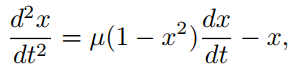
\includegraphics[width=0.4\linewidth]{vandePol}
		\caption{}
		\label{fig:vandepol}
	\end{figure}
	a) Bằng việc đặt ẩn phụ, hãy chuyển hệ bậc hai về hệ bậc nhất.\\ 
	b) Giải bài toán giá trị ban đầu trên đoạn $[0,100]$ với các giá trị khác nhau của $\mu = 10, 100, 500, 1000$
	với điều kiện ban đầu $x(0)=x'(0)=1$ sử dụng ít nhất 2 phương pháp ẩn và hai phương pháp hiện đã học.  \\
	c) So sánh tính hiệu quả của các phương pháp các em đã trình bày ở phần b). 
\end{bt}

\begin{bt}
	Độ nhớt của một chất lưu là thông số đại diện cho ma sát trong của dòng chảy được biểu diễn qua một hàm số của nhiệt độ T. 
	%
	\begin{center}
		\begin{tabular}[7]{l|l|l|l|l|l|l|l}
			T & 1    & 2    & 3    & 4    & 5    & 6    & 7 \\ \hline
			V & 2.31 & 2.01 & 1.80 & 1.66 & 1.55 & 1.47 & 1.41.
		\end{tabular}	
	\end{center}
	% 
	Sử dụng 2 phương pháp spline bậc 3 (cubic spline) và spline bậc 3 tự nhiên (natural cubic spline) để nội suy trên đoạn $[1,7]$ và vẽ hàm $V(T)$. 
\end{bt}

\centerline{———————————Hết——————————-}

%\end{document}

\vspace{1cm}
\noindent{\bf Chú ý:} {\it Cán bộ coi thi không giải thích gì thêm}\\
\Closesolutionfile{ans}
\newpage
\begin{center}
{\LARGE{\bf ĐÁP ÁN}}
\end{center}


\end{document}



